\documentclass[11pt]{article}
\usepackage[margin=1in]{geometry}
\usepackage[T1]{fontenc}
\usepackage{lmodern}
\usepackage{amsmath,amssymb,amsthm}
\usepackage{graphicx}
\usepackage[colorlinks=true,linkcolor=blue,citecolor=blue,urlcolor=blue]{hyperref}
\emergencystretch=3em

\newtheorem{theorem}{Theorem}
\newtheorem{remark}{Remark}

\title{Rotation-Invariant Positive Kernels Defeat\
Two Abstract Rigidity Questions}
\author{Run \texttt{fa\_banach\_001}}
\date{2026-08-13}

\begin{document}
\maketitle

\noindent\textbf{Status.}
Candidate full counterexamples, likely valid, to Questions 5.1 and 5.4 in
the source paper.

\section{Source questions}
Bilokopytov calls a nondegenerate kernel $K$ projectively invariant under a
group action if, for every group element $g$, the transformed kernel
$K(g\cdot z,g\cdot w)$ is a rescaling of $K$.  A multiplier is a nonvanishing
function implementing that rescaling; it is naturally determined only up to
a constant unimodular factor.

Question 5.1 asks whether two nondegenerate positive semidefinite continuous
kernels on a transitive topological $G$-space, both projectively invariant
and having equal multipliers, must satisfy $L=cK$ for some $c>0$
\cite{Bilokopytov}.

\begin{center}
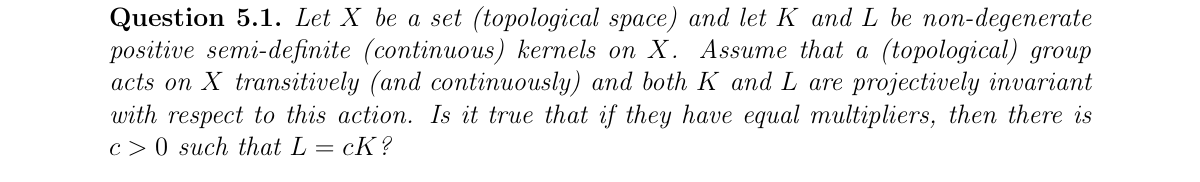
\includegraphics[width=0.98\linewidth]{figures/open_problem_q51_crop.png}
\end{center}

Question 5.4 asks whether a separately continuous, positive semidefinite,
nondegenerate kernel must be constant if $G$ acts transitively and
continuously and
\[
 K(g\cdot x,g\cdot y)=e^{\alpha(g)}K(x,y)
\]
for a continuous homomorphism $\alpha:G\to\mathbb R$
\cite{Bilokopytov}.

\begin{center}
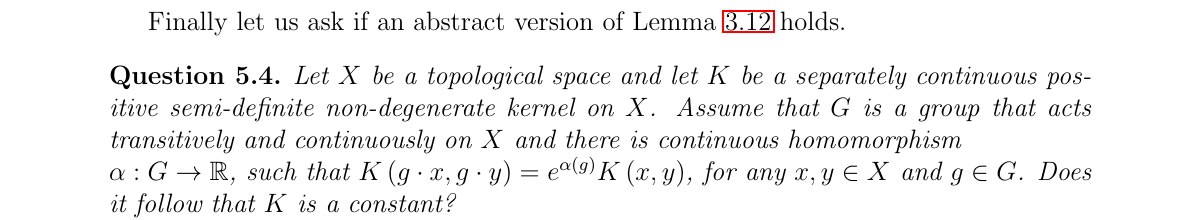
\includegraphics[width=0.98\linewidth]{figures/open_problem_q54_crop.png}
\end{center}

\section{Idea of the proof}
Positive definiteness is compatible with a large supply of invariant
kernels: every unitary representation gives matrix-coefficient kernels.
The smallest connected example already suffices.  On the circle, the two
features $1$ and $\sqrt a\,z$ give the positive kernel
$K_a(z,w)=1+a z\overline w$.  Rotating both variables cancels the two phase
factors, so every member of the family has the same trivial multiplier.
Changing $a$ changes the kernel without changing the symmetry data.  This is
exactly the freedom that sesqui-holomorphic rigidity removed in the theorem
preceding Question 5.1.

\section{Counterexample theorem}
\begin{theorem}
Let
\[
 X=G=\mathbb T=\{z\in\mathbb C:|z|=1\},\qquad
 g\cdot z=gz,
\]
with their usual topologies.  For $0<a<1$, define
\[
 K_a(z,w)=1+a z\overline w.
\]
Then:
\begin{enumerate}
\item $K_a$ is a continuous, nondegenerate, positive semidefinite kernel,
      is nowhere zero, and is exactly $G$-invariant;
\item for every $g\in G$, the complete family of multipliers rescaling
      $K_a(g\cdot z,g\cdot w)$ to $K_a(z,w)$ consists of the constant
      unimodular functions, independently of $a$;
\item if $0<a<b<1$, then $K_b$ is not a positive scalar multiple of $K_a$.
\end{enumerate}
Consequently, $(K_a,K_b)$ is a counterexample to Question 5.1.  Moreover,
$(X,G,K_a,\alpha)$ with $\alpha\equiv0$ is a counterexample to Question 5.4.
\end{theorem}

\begin{proof}
The rotation action is continuous and transitive.  For arbitrary
$z_1,\ldots,z_N\in\mathbb T$ and $c_1,\ldots,c_N\in\mathbb C$,
\begin{align*}
 \sum_{i,j=1}^N c_i\overline{c_j}K_a(z_i,z_j)
 &=\left|\sum_{i=1}^N c_i\right|^2
   +a\left|\sum_{i=1}^N c_i z_i\right|^2\geq0.
\end{align*}
Thus $K_a$ is positive semidefinite.  It is continuous, and
$K_a(z,z)=1+a>0$, so it is nondegenerate in the source's sense.  Also
\[
 |K_a(z,w)|=|1+a z\overline w|\geq1-a>0,
\]
so it never vanishes.

For $g\in\mathbb T$,
\[
 K_a(gz,gw)=1+a(gz)\overline{gw}
            =1+a z\overline w=K_a(z,w).
\]
Hence $K_a$ is projectively invariant, and the constant function $1$ is a
multiplier for every rotation.

We also verify the stronger, convention-independent statement about the
whole multiplier class.  Suppose a nonvanishing function $\omega$ rescales
the transformed kernel to the original one.  Exact invariance gives
\[
 \omega(z)\overline{\omega(w)}K_a(z,w)=K_a(z,w)
 \qquad(z,w\in\mathbb T).
\]
Since $K_a$ is nowhere zero,
$\omega(z)\overline{\omega(w)}=1$ for all $z,w$.  Taking $z=w$ gives
$|\omega(z)|=1$, and then varying $z,w$ shows that $\omega$ is constant.
Conversely every constant unimodular function works.  The multiplier class
therefore does not depend on $a$.

If $K_b=cK_a$ for $c>0$, evaluating at $(z,w)=(1,1)$ and $(1,-1)$ yields
\[
 1+b=c(1+a),\qquad 1-b=c(1-a).
\]
Eliminating $c$ gives
$(1+b)(1-a)=(1-b)(1+a)$, hence $2(b-a)=0$, contrary to $a<b$.
This proves the counterexample to Question 5.1.

Finally take any $0<a<1$ and $\alpha(g)=0$.  This is a continuous
homomorphism $\mathbb T\to\mathbb R$, and exact invariance gives the covariance
identity in Question 5.4.  But
\[
 K_a(1,1)=1+a\neq1-a=K_a(1,-1),
\]
so $K_a$ is not a constant function on $X\times X$.  Question 5.4 is
therefore also answered negatively.
\end{proof}

\section{Verification and robustness}
The proof checks every printed hypothesis directly.  The same example works
on a connected compact space with a connected compact acting group, so the
failure is not caused by discreteness.  Restricting to $0<a<1$ is not needed
for positive semidefiniteness, but it makes the kernel nowhere zero and
removes any ambiguity about the full multiplier class.

The script \texttt{code/verify\_rotation\_kernels.py} samples finite Gram
matrices, rotations, and scalar-multiple tests for several parameters.  It is
only a sanity check; positive semidefiniteness and all identities are proved
symbolically above.  The independent audit is recorded in
\texttt{VERIFICATION.md}.

\section{Scope and novelty check}
This packet settles only the two abstract Questions 5.1 and 5.4.  It does not
answer the paper's Questions 5.2 or 5.3, nor its broader classification of
automorphism-invariant pull-back metrics on complex domains.

A bounded search on 2026-08-13 used arXiv:1711.05211, the exact title and
author, the exact phrases ``equal multipliers'' and ``does it follow that
$K$ is a constant'', and projectively invariant positive-kernel keywords.
It found the source, the author's dissertation repeating the surrounding
program, and general literature on projectively invariant kernels, but no
later source explicitly answering Questions 5.1 or 5.4.  Novelty confidence
is moderate; mathematical-validity confidence is high because the example is
elementary and all assumptions are verified directly.

\enlargethispage{4\baselineskip}
\begin{thebibliography}{9}
\bibitem{Bilokopytov}
E. Bilokopytov,
\emph{Invariant Hermitean Metric Generated By Reproducing Kernel Hilbert
Spaces}, arXiv:1711.05211v3 (2018), Questions 5.1 and 5.4.
\end{thebibliography}

\end{document}
